
\subsection*{Hint for Review Question~\ref{leftright}}

%%%Insert this to get the typewriter font so it looks like a real movie script
{\ttfamily
\fontdimen2\font=0.4em
\fontdimen3\font=0.2em
\fontdimen4\font=0.1em
\fontdimen7\font=0.1em
\hyphenchar\font=`\-


\hypertarget{inverse_matrix_hint}{In} 
the text, only inverses for square matrices were discussed, but there is a notion of left and right inverses for matrices that are not square.
It helps to look at an example with bits to see why.
To start with we look at vector spaces
\[{\mathbb Z}_2^3=\{(x,y,z)|x,y,z=0,1\}\qquad \mbox{ and } \qquad {\mathbb Z}_2^2=\{(x,y)|x,y=0,1\}\, .\]
These have 8 and 4 vectors, respectively, that can be depicted as corners of a cube or square:
\begin{center}
${\mathbb Z}_2^3$\raisebox{-15mm}{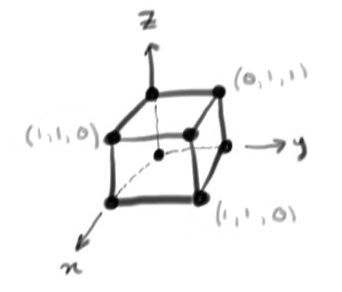
\includegraphics[alt={The cube in three dimensions with each vertex at 0 or 1 for each coordinate axis.},scale=0.5]{Z23.jpg}} \hspace{4mm} or ${\mathbb Z}_2^2$\raisebox{-10mm}{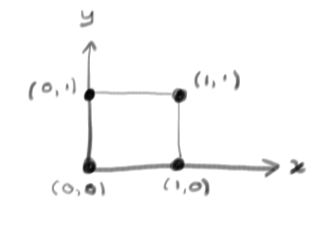
\includegraphics[alt={The square in two dimensions with vertices (0,0), (0,1), (1,0), and (1,1).},scale=0.5]{Z22.jpg}}
\end{center}
Now lets consider a linear transformation
\[
L:{\mathbb Z}_2^3\longrightarrow{\mathbb Z}_2^2\, .
\]
This must be represented by a matrix, and lets take the example
\[
L\begin{pmatrix}x\\y\\z\end{pmatrix}=\begin{pmatrix}0 & 1 & 1\\1 & 1 &0\end{pmatrix}\begin{pmatrix}x\\y\\z\end{pmatrix}:=A X\, .
\]
Since we have bits, we can work out what $L$ does to every vector, this is listed below
\[
\begin{array}{ccc}
(0,0,0)&\stackrel{L}\mapsto&(0,0)\\[2mm]
(0,0,1)&\stackrel{L}\mapsto&(1,0)\\
(1,1,0)&\stackrel{L}\mapsto&(1,0)\\[2mm]
(1,0,0)&\stackrel{L}\mapsto&(0,1)\\
(0,1,1)&\stackrel{L}\mapsto&(0,1)\\[2mm]
(0,1,0)&\stackrel{L}\mapsto&(1,1)\\
(1,0,1)&\stackrel{L}\mapsto&(1,1)\\
(1,1,1)&\stackrel{L}\mapsto&(1,1)
\end{array}
\]
Now lets think about left and right inverses. A left inverse $B$ to the matrix $A$
would obey
\[
BA=I
\]
and since the identity matrix is square, $B$ must be $2\times3$. It would have to undo the action of $A$ and return vectors in ${\mathbb Z}_2^3$
to where they started from. But above, we see that different vectors in ${\mathbb Z}_2^3$ are mapped to the same vector in ${\mathbb Z}_2^2$
by the linear transformation $L$ with matrix $A$. So $B$ cannot exist. However a right inverse $C$ obeying
\[
AC=I
\]
can. It would be $2\times2$. Its job is to take a vector in ${\mathbb Z}_2^2$ back to one in ${\mathbb Z}_2^3$ in a way that gets undone by the action of $A$.
This can be done, but not uniquely. 

} % Closing bracket for font

%\newpage
